Este capítulo se corresponde con la segunda etapa de la metodología CRISP-DM, En el se explicará la naturaleza de los datos y sus características, así como los valores atípicos que presentan y sus sesgos.

\section{Origen de los datos}  \label{sec.origen-datos}
Para elegir un conjunto de datos que se adapte a las necesidades de los modelos de clasificación que se desarrollan en este trabajo, se realizó una búsqueda y comparación entre diferentes \textit{datasets} que contienen datos de conexiones benignas y malignas a sistemas informáticos. Algunos de los datasets descartados son:

\begin{itemize}
	\item \texttt{KDD 1999}: es un conjunto de datos creado para la detección de intrusiones en redes, derivado de \texttt{DARPA 1998}. Este \textit{dataset} contiene tráfico simulado con etiquetas de ataques y tráfico normal. Su uso fue descartado para este trabajo por estár desactualizado, tener datos redundantes y no reflejar las amenazas modernas ni el tráfico real de las redes actuales. \href{https://www.kaggle.com/datasets/sampadab17/network-intrusion-detection/data?select=Test_data.csv}{Ver el conjunto de datos}.
	\item \texttt{CIC-IDS-2017}: es un conjunto de datos generado por la \href{https://www.unb.ca/cic/datasets/ids-2017.html}{Universidad de Brunswick}. El \textit{dataset} se divide 8 ficheros CSV y presenta una escasa variedad de tipos de ataques, lo que no es representativo del tráfico real actual. Además, en ciberseguridad, los tipos de ataques y su funcionamiento varian cada muy poco tiempo, lo que implica que un conjunto de datos con 8 años ya se considera desactualizado. \href{https://www.kaggle.com/datasets/chethuhn/network-intrusion-dataset}{Ver el conjunto de datos}.
	\item \texttt{MIT-datasets}: el \href{https://www.ll.mit.edu/r-d/datasets?author=All&rdarea=All&rdgroup=All&keywords=cyber&tag=All&items_per_page=100}{Instituto de Tecnología de Massachusetts} (MIT) cuenta con varios \textit{dataset} con información sobre conexiones malignas en redes. Algunos de ellos se basan en \texttt{DARPA}. La mayoria de los conjuntos de datos son antiguos y no detallan como se obtuvo la información que los compone, por estos motivos, estos \textit{datasets} también fueron descartados. \href{https://archive.ll.mit.edu/ideval/index.html}{Ver el conjunto de datos}.
\end{itemize}

Tras comparar varios conjuntos de datos, los datos que se utilizan para desarrollar este trabajo, se han obtenido de  conjuntos de datos diseñados para entrenar Sistemas de Detección de Intrusión de Red (NIDS) basados en el aprendizaje automático. El conjunto de datos en cuenstión  forma parte de un análisis realizado en la \href{https://staff.itee.uq.edu.au/marius/NIDS_datasets/}{Universidad de Queensland}, Australia \cite{luay2025NetFlowDatasetsV3}.

El \textit{dataset} utilizado es \texttt{NF-UNSW-NB15-v3}, se trata de una versión basada en \texttt{NetFlow} del conjunto de datos \texttt{UNSW-NB15}, mejorado con características adicionales de \texttt{NetFlow} y etiquetada de acuerdo con sus respectivas categorías de ataque. Su última actualización es del año 2025 y cuenta con una gran variedad de tipos de ataques registrados entre sus datos.

La Universidad de Queensland cuenta con otros \textit{datasets} con características similares, pero de entre los conjuntos de datos desarrollados por esta entidad el más completo y actualizado es el que finalmente se ha elegido para desarrollar los modelos de este proyecto.

\section{Tipos de ataques registrados en los datos de \texttt{NF-UNSW- NB15-v3}} \label{sec.tipo-ataques}
En esta sección se explican los tipos de datos presentes en el \textit{dataset} que se utiliza para entrenar a los modelos del proyecto. Se explica en que consiste cada tipo de ataque registrado así como el número exacto de ataques de cada tipo presente.

El conjunto de datos consiste en un total de 2\,365\,424 flujos de datos, donde 127\,639 (5,4\%) son muestras de ataque y 2\,237\,731 (94,6\%) son benignos. Los flujos de ataque se clasifican en nueve clases, cada una representando una amenaza a la red distinta. La Tabla \ref{tab:attacks-tab} proporciona una distribución detallada del conjunto de datos:

\begin{table}[H]
\begin{tabular}{|l|c|>{\RaggedRight}p{8cm}|} % Ajusta el ancho (8cm) según necesites
\hline
\rowcolor[HTML]{C0C0C0} 
\textbf{Clase} & \textbf{Cantidad} & \textbf{Descripción} \\ \hline
Benigno & 2\,237\,731 & Flujos normales no maliciosos. \\ \hline
\textit{Fuzzers} & 33\,816 & Tipo de ataque en el que el atacante envía grandes cantidades de datos aleatorios que hacen que un sistema se bloquee y también apuntan a descubrir vulnerabilidades de seguridad en un sistema. \\ \hline
\textit{Analysis} & 2\,381 & Un grupo que presenta una variedad de amenazas que se dirigen a aplicaciones web a través de puertos, correos electrónicos y \textit{scripts}. \\ \hline
\textit{Backdoor} & 1\,226 & Una técnica que tiene como objetivo eludir los mecanismos de seguridad respondiendo a aplicaciones específicas de clientes construidos. \\ \hline
DoS & 5\,980 & La denegación de servicio es un intento de sobrecargar los recursos de un sistema informático con el objetivo de evitar el acceso o la disponibilidad de sus datos. \\ \hline
\textit{Exploits} & 42\,748 & Son secuencias de comandos que controlan el comportamiento de un \textit{host} a través de una vulnerabilidad conocida. \\ \hline
\textit{Generic} & 19\,651 & Un método que se dirige a la criptografía y causa una colisión con cada cifrado de bloques. \\ \hline
\textit{Reconnaissance} & 17\,074 & Una técnica para recopilar información sobre un \textit{host} de red, también se conoce como sonda. \\ \hline
\textit{Shellcode} & 4\,659 & Un \textit{malware} que penetra en un código para controlar el \textit{host} de una víctima. \\ \hline
\textit{Worms} & 158 & Ataques que se replican y se extienden a otros sistemas. \\ \hline
\end{tabular}
\centering
\caption{Clasificación de amenazas de seguridad del dataset \texttt{NF-UNSW-NB15-v3}.} 
\label{tab:attacks-tab}
\end{table}

\section{Parámetros de los datos} \label{sec.param-datos}
En esta sección se explicarán el significado de cada uno de los 55 atributos que componen cada fila del \textit{dataset} seleccionado. El \textit{dataset}, que es de dominio público se puede descargar en formato .csv donde los atributos se encuentran separados por comas \cite{luay2025NetFlowDatasetsV3}.

\begin{enumerate}
    \item \texttt{IPV4\_SRC\_ADDR}: Dirección IPv4 de origen.
    \item \texttt{IPV4\_DST\_ADDR}: Dirección IPv4 de destino.
    \item \texttt{L4\_SRC\_PORT}: Número de puerto de origen de la capa 4.
    \item \texttt{L4\_DST\_PORT}: Número de puerto de destino de la capa 4.
    \item \texttt{PROTOCOL}: Byte identificador del protocolo IP.
    \item \texttt{L7\_PROTO}: Protocolo que opera en la capa 7 del Modelo OSI, también conocida como capa de aplicación.
    \item \texttt{IN\_BYTES}: Número de bytes entrantes.
    \item \texttt{OUT\_BYTES}: Número de bytes salientes.
    \item \texttt{IN\_PKTS}: Número de paquetes entrantes.
    \item \texttt{OUT\_PKTS}: Número de paquetes salientes.
    \item \texttt{FLOW\_DURATION\_MILLISECONDS}: Duración del flujo en ms.
    \item \texttt{TCP\_FLAGS}: \textit{Bits} dentro del encabezado TCP que indican el estado o la dirección de una conexión TCP.
    \item \texttt{CLIENT\_TCP\_FLAGS}: \textit{Bits} dentro del encabezado TCP que indican el estado de la conexión TCP del cliente.
    \item \texttt{SERVER\_TCP\_FLAGS}: \textit{Bits} dentro del encabezado TCP que indican el estado de la conexión TCP del servidor.
    \item \texttt{DURATION\_IN}: Duración del flujo Cliente a Servidor (ms).
    \item \texttt{DURATION\_OUT}: Duración del flujo Cliente a Servidor (ms).
    \item \texttt{MIN\_TTL}: Mínimo valor del TTL (\textit{Time To Live}), que limita la duración de un paquete de datos en una red informática, durante la sesión TCP.
    \item \texttt{MAX\_TTL}: Maximo valor del TTL (\textit{Time To Live}), que limita la duración de un paquete de datos en una red informática, durante la sesión TCP.
    \item \texttt{LONGEST\_FLOW\_PKT}: Paquete de mayor tamaño enviado durante la conexión de los sistemas (bytes).
    \item \texttt{SHORTEST\_FLOW\_PKT}: Paquete de menor tamaño enviado durante la conexión de los sistemas (bytes)
    \item \texttt{MIN\_IP\_PKT\_LEN}: Longitud del paquete IP más pequeño del flujo observado.
    \item \texttt{MAX\_IP\_PKT\_LEN}: Longitud del paquete IP más grande del flujo observado.
    \item \texttt{SRC\_TO\_DST\_SECOND\_BYTES}: \textit{Bytes}/segundo de origen a destino.
    \item \texttt{DST\_TO\_SRC\_SECOND\_BYTES}: \textit{Bytes}/segundo de destino a origen.
    \item \texttt{RETRANSMITTED\_IN\_BYTES}: Número de bytes TCP retransmitidos del flujo (src a dst).
    \item \texttt{RETRANSMITTED\_IN\_PKTS}: Número de paquetes TCP retransmitidos del flujo (src a dst).
    \item \texttt{RETRANSMITTED\_OUT\_BYTES}: Número de bytes TCP retransmitidos del flujo (dst a src).
    \item \texttt{RETRANSMITTED\_OUT\_PKTS}: Número de paquetes TCP retransmitidos del flujo (dst a src).
    \item \texttt{SRC\_TO\_DST\_AVG\_THROUGHPUT}: Tasa de transferencia promedio de origen a destino (bps).
    \item \texttt{DST\_TO\_SRC\_AVG\_THROUGHPUT}: Tasa de transferencia promedio de destino a origen (bps).
    \item \texttt{NUM\_PKTS\_UP\_TO\_128\_BYTES}: Paquetes cuyo tamaño IP es $ \leq $ 128.
    \item \texttt{NUM\_PKTS\_128\_TO\_256\_BYTES}: Paquetes cuyo tamaño IP es  $ > $ 128 y $ \leq $ 256.
    \item \texttt{NUM\_PKTS\_256\_TO\_512\_BYTES}: Paquetes cuyo tamaño IP es $ > $ 256 y $ \leq $ 512.
    \item \texttt{NUM\_PKTS\_512\_TO\_1024\_BYTES}: Paquetes cuyo tamaño IP es $ > $ 512 y $ \leq $ 1024.
    \item \texttt{NUM\_PKTS\_1024\_TO\_1514\_BYTES}: Paquetes cuyo tamaño IP es $ > $ 1024 y $ \leq $ 1514.
    \item \texttt{TCP\_WIN\_MAX\_IN}: Ventana TCP máxima (src a dst).
    \item \texttt{TCP\_WIN\_MAX\_OUT}: Ventana TCP máxima (dst a src).
    \item \texttt{ICMP\_TYPE}: Tipo ICMP * 256 + Código ICMP.
    \item \texttt{ICMP\_IPV4\_TYPE}: Tipo ICMP.
    \item \texttt{DNS\_QUERY\_ID}: ID de transacción de la consulta DNS.
    \item \texttt{DNS\_QUERY\_TYPE}: Tipo de consulta DNS (ej., 1=A, 2=NS..).
    \item \texttt{DNS\_TTL\_ANSWER}: TTL del primer registro A (si existe).
    \item \texttt{FTP\_COMMAND\_RET\_CODE}: Código de retorno del comando del cliente FTP.
    \item \texttt{FLOW\_START\_MILLISECONDS}: Marca de tiempo de inicio del flujo en ms.
    \item \texttt{FLOW\_END\_MILLISECONDS}: Marca de tiempo de fin del flujo en ms.
    \item \texttt{SRC\_TO\_DST\_IAT\_MIN}: IAT mínimo (src a dst).
    \item \texttt{SRC\_TO\_DST\_IAT\_MAX}: IAT máximo (src a dst).
    \item \texttt{SRC\_TO\_DST\_IAT\_AVG}: IAT promedio (src a dst).
    \item \texttt{SRC\_TO\_DST\_IAT\_STDDEV}: Desviación estándar del IAT (src a dst).
    \item \texttt{DST\_TO\_SRC\_IAT\_MIN}: IAT mínimo (dst a src).
    \item \texttt{DST\_TO\_SRC\_IAT\_MAX}: IAT máximo (dst a src).
    \item \texttt{DST\_TO\_SRC\_IAT\_AVG}: IAT promedio (dst a src).
    \item \texttt{DST\_TO\_SRC\_IAT\_STDDEV}: Desviación estándar del IAT (dst a src).
\end{enumerate}

Este conjunto de datos ya se encontraba previamente etiquetado, lo que permite realizar un trabajo como el propuesto en el tiempo establecido. Típicamente, los conjuntos de datos enfocados a la clasificación suelen tener una única etiqueta, pero este conjunto de datos tiene dos, lo que agiliza el tratamiento del conjunto de los datos para el entrenamiento y la evaluación de los modelos que se proponen en este proyecto.

\begin{enumerate}
    \item \texttt{Label}: Toma valor 0 si el flujo es benigno y 1 si se trata de un ataque.
    \item \texttt{Attack}: Clase de flujo, perteneciente a las clases mencionadas en \ref{tab:attacks-tab} \nameref{tab:attacks-tab}
\end{enumerate}

\section{Selección de atributos}\label{sec:selectdatos}
En esta sección se comentan los atributos prelinimares, así como los valores y los sesgos presentes en el \textit{dataset}. La identificación de estas irregularidades es fundamental para el correcto desarrollo del proyecto.

Al analizar los datos originales del \textit{dataset}, se encuentran características que afectan de forma negativa al entrenamiento del modelo y por lo tanto, a su correcto funcionamiento. A continuación, se mencionan cuales son las características problematicas de los datos que se utilizan.


Tras estudiar los datos, se descubre que algunos parámetros presentan valores infinitos, estos valores alteran la distribución inherente de las variables, introduciendo valores que no se pueden tratar en el proceso de aprendizaje. Los algoritmos de entrenamiento, diseñados para operar con valores numéricos finitos, pueden comportarse de manera impredecible o inestable ante la presencia de infinitos, dificultando la convergencia hacia una solución óptima. Asimismo, la interpretación de las características con valores infinitos se vuelve ambigua, comprometiendo la capacidad del modelo para establecer relaciones significativas con otras variables y para generalizar correctamente a datos futuros que no contengan tales valores extremos. En consecuencia, la presencia de infinitos puede degradar sustancialmente el rendimiento y la fiabilidad del modelo entrenado.

Como se comenta en la sección anterior \ref{sec.param-datos} \nameref{sec.param-datos}, existen dos parámetros que registran la IP origen y la IP destino de la conexión. En principio, si los datos no fuesen sintéticos, la dirección IP de la máquina que origina la comunicación sería aleatoria. En este conjunto de datos, se puede observar como todos los ataques provienen de IP con máscara 175.45.176.255, lo que no encaja con la realiadad. Independientemente de este patrón, que no se manifiesta de forma natural en las conexiones entre sistemas, el uso de las IPs de las máquinas en el entranamiento de los modelos provoca que el algoritmo encargado de este entrenamiento asigne pesos de manera incorrecta a un parámetro que no influye en la clasificación que se propone para este trabajo.



\section{Preparación de los datos}\label{sec.prep-datos}
En esta sección se modificarán los datos que presentan patrones, valores atípicos o sesgos que se comentan en la sección anterior, \ref{sec:selectdatos} \nameref{sec:selectdatos}. Así como el tratamiento necesario de los datos para poder entrenar los modelos.

Una de las características problemáticas, es la existencia de parámetros con valores infinito. Para tratar con esta problemática existen dos enfoques, o bien se sustituyen los valores infinitos por el máximo valor posible para ese parámetro, o bien, se elimina el flujo al que pertenece cada valor infinito. Para este trabajo, se opta por eliminar los registros con valores infinitos, ya que asginarles un valor falso, podría crear una relación sintética entre los datos y provocar que el modelo no converja en una solución real.

Para entrenar un modelo es necesario que en primer lugar todos los parámetros sean numéricos. En los datos originales del \textit{dataset}, se encuentran tres parámetros que no presentan un formato numérico: \texttt{IPV4\_SRC\_ADDR}, \texttt{IPV4\_DST\_ADDR} y \texttt{Attack}.

\begin{itemize}
	\item Para dar un formato correcto al parámetro \texttt{Attack}, se utiliza el codificador \texttt{LabelEncoder} de la biblioteca sklearn.preprocessing y el método \texttt{fit\_transform} de la biblioteca \texttt{sklearn}. La primera función, \texttt{LabelEncoder} codifica las etiquetas de características categóricas en valores numéricos entre 0 y el número de clases menos 1. Una vez se instancian las categorías del parámtero, el método \texttt{fit\_transform} permite entrenar el codificador y transformar el conjunto de datos en un único paso.
	\item Las direcciones IPv4 están formadas por cuatro octetos separados por puntos. Obviamnete este formato no es numérico, por ese motivo se opta por dividir las direcciones IPv4 en 4 parámetros diferentes, uno por cada octeto. De esta manera, si el valor de un flujo para el parámetro \texttt{IPV4\_SRC\_ADDR} es 175.45.176.23, se separa en cuatro nuevos valores que son: 175, 45, 176 y 23. Para realizar esta transformación se utiliza la función \ref{fig:funIPv4} \nameref{fig:funIPv4}.
\begin{figure}[H]
    \centering
    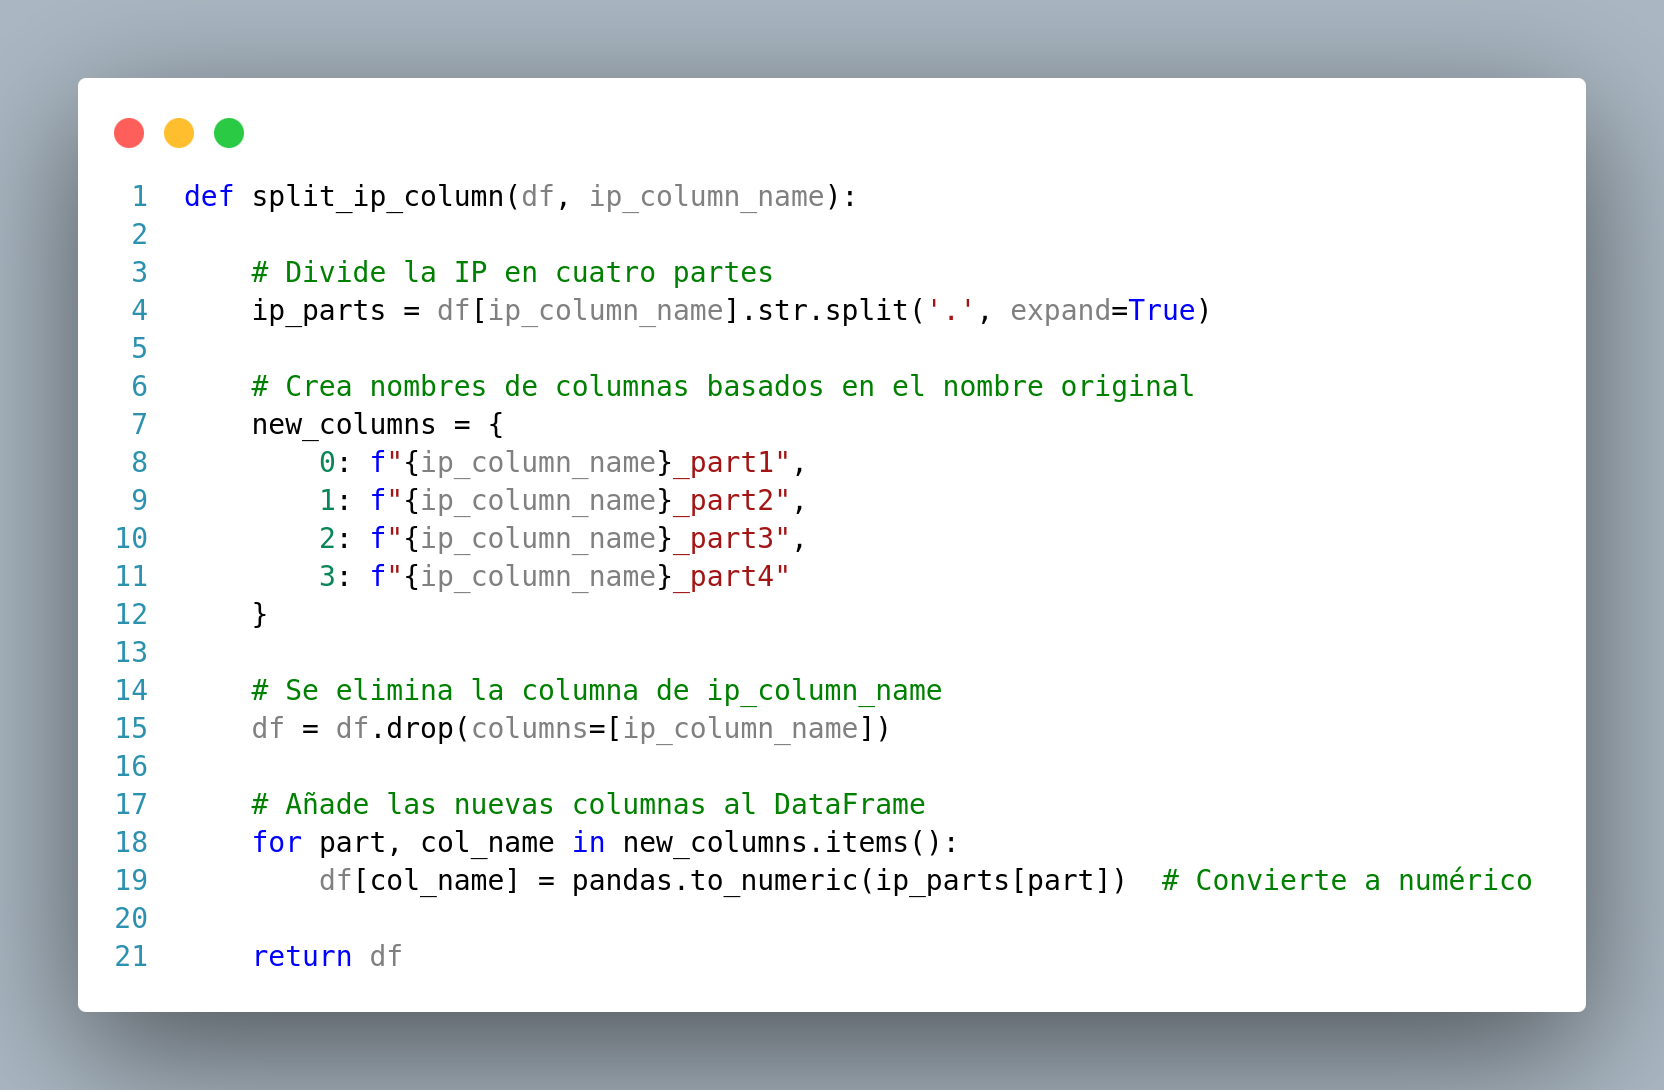
\includegraphics[width=0.8\textwidth]{./img/ent-datos/funIPv4.png}
    \caption{Función de transformación para los parámetros IPv4.}
    \label{fig:funIPv4}
\end{figure}

\end{itemize}

Una vez que todos los parámetros presentan valores numéricos, se separan los parámetros ente los que formarán parte de la entrada del modelo neuronal como atributos (a partir de ahora se les menciona como X) y los que contienen el valor de la salida que debe proporcionar el modelo neuronal llamados etiquetas(a partir de ahora se les menciona como Y).

Los parámetros que pertenecen a Y son \texttt{Label} y \texttt{Attack}. Sin embargo, en función del modelo que se entrena se utiliza o bien \texttt{Label}, o bien \texttt{Attack}, pero nunca los dos al mismo tiempo.

Por su parte, X la conforman el total de los parámetros del \textit{dataset} a excepción de:
\begin{itemize}
	\item \textbf{\texttt{Label} y \texttt{Attack}}: Se trata de los parámetros que conforman Y o etiquetas, si estos parámetros formasen parte de los datos de entrada del modelo, el algoritmo encargado de entrenarlo, les asignaría a estos parámetros unos pesos muy elevados y tendría una tasa teórica de éxito del 100\%, puesto que, se estaría introduciendo la respuesta al problema que se aborda directamente como entrada al modelo. En un sistema informático real esta práctica es imposible.
	\item \textbf{\texttt{IPV4\_SRC\_ADDR} y \texttt{IPV4\_DST\_ADDR}}: Tal y como se menciona en la sección \ref{sec.param-datos} \nameref{sec.param-datos}, estos parámetros presentan un patrón irregular y sintético. Al introducir estos parámetros como entradas para el entrenamiento del modelo, de forma análoga a como sucede con los parámetros \texttt{Label} y \texttt{Attack} se estarían introduciendo valores que no se pueden obtener en una situación realista y condicionando el comportamiento del modelo. Esto implica como se menciona en los siguiente capítulos que el modelo resultante obtendría muy buenas métricas en validación pero muy malas al someterlo a datos que nunca ha visto durante su entrenamiento.
	\item \textbf{\texttt{FLOW\_START\_MILLISECONDS} y \texttt{FLOW\_END\_MILLISECONDS}}: A diferencia de los anteriores parámetros, estos muestran valores que puedan condicionar el entrenamiento de los modelos ni sus resultados, pero se trata de parámetros que ofrecen información redundante, pues el parámetro \texttt{FLOW\_DURATION\_MILLISECONDS} es combinación lineal de estos dos. Al eliminar estos parámetros se agiliza el entrenamiento del modelo y su tiempo de respuesta una vez entrenado sin perjudicar su precisión.
\end{itemize}

Como el conjunto de datos original presentaba 53 atributos de entrada a los modelos y se ha descartado el uso de 4 de ellos, los modelos serán entrenados con 49 atributos de entrada. 

Para finalizar con el tratamiento de los datos, se normalizan los valores de X para que no haya tanta varianza entre los parámetros que lo conforman. Para normalizar los valores se utiliza el escalador \texttt{MinMaxScaler} que forma parte de la biblioteca \texttt{sklearn.preprocessing} junto con el método \texttt{fit\_transform} que se menciona en la explicación de la transformación del parámetro \texttt{Attack}. Llamando a \texttt{MinMaxScaler} con un rango (0,1), tras haber tratado los datos con el método \texttt{fit\_transform}, se obtienen valores escalados en un rango entre 0 y 1, lo que facilita la comparación y el procesamiento por parte de los algoritmos de aprendizaje automático sin alterar las relaciones proporcionales inherentes en los datos originales.
